\documentclass[tikz,border=1mm]{standalone}
\usetikzlibrary{arrows.meta, positioning}

\begin{document}
	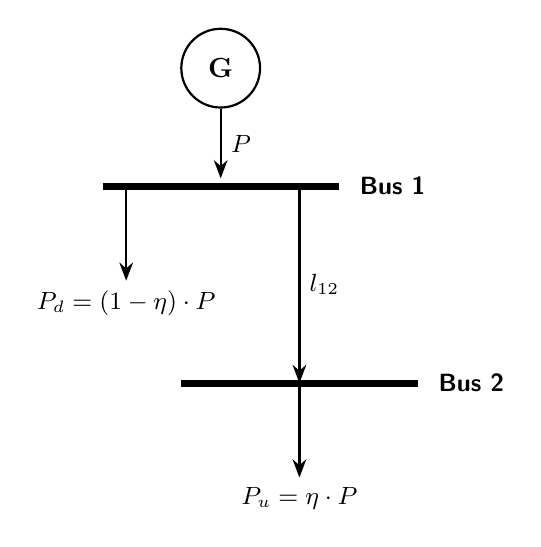
\begin{tikzpicture}[
		% Estilo para las barras (Buses)
		bus/.style={line width=2.5pt, draw=black},
		% Estilo para el generador (Círculo de potencia)
		generador/.style={draw, circle, minimum size=1.0cm, fill=white, thick},
		flecha/.style={-Stealth, thick},
		etiqueta/.style={font=\small\sffamily}
		]
		
		% --- BARRA 1 (Bus 1 - Superior) ---
		% Barra 1 horizontal
		\draw[bus] (0,0) -- (3,0) node[right=3pt, etiqueta] {\textbf{Bus 1}};
		
		% Generador inyectando potencia P desde arriba
		\node[generador] (gen) at (1.5,1.5) {};
		%\draw[thick] (1.25,1.5) sin (1.5,1.65) cos (1.75,1.5); % Onda senoidal
		\draw[flecha] (gen) -- (1.5,0.1) node[midway, right, etiqueta] {$P$};
		\node at (1.5,1.5) {\textbf{G}}; % Letra G centrada
		% Flecha de carga/pérdida Pr1 saliendo por el extremo izquierdo hacia abajo
		\draw[flecha] (0.3,0) -- (0.3,-1.2) node[below, etiqueta] {$P_{d} = (1 - \eta) \cdot P$};
		
		
		% --- LÍNEA DE TRANSMISIÓN (HACIA ABAJO) ---
		% Conexión vertical entre Bus 1 y Bus 2
		\draw[flecha] (2.5,0) -- (2.5,-2.5) node[midway, right, etiqueta] {$l_{12}$};
		
		
		% --- BARRA 2 (Bus 2 - Inferior) ---
		% Barra 2 horizontal, alineada con la línea de transmisión
		\draw[bus] (1,-2.5) -- (4,-2.5) node[right=3pt, etiqueta] {\textbf{Bus 2}};
		
		% Flecha de carga/pérdida Pr2 saliendo del Bus 2 hacia abajo
		\draw[flecha] (2.5,-2.5) -- (2.5,-3.7) node[below, etiqueta] {$P_{u} = \eta \cdot P$};
		
	\end{tikzpicture}
\end{document}
